\section{Experimental Protocol}
\label{sec:protocol}

\subsection{Data, Models and Operating Points}

The tasks classify benign versus attack flows from the corrected
\texttt{CICIDS2017\_improved} re-extraction~\cite{engelen2021troubleshooting,liu2022error}
and the \texttt{NF-ToN-IoT-V2} NetFlow release~\cite{sarhan2022towards}.
Table~\ref{tab:protocol} specifies the retained matrices and selected models.
Preparation removes non-finite rows, clips features at $10^{12}$ and caps each
class at 250,000 rows. Exact clipped \texttt{float64} feature hashes define
groups; conflicting-label groups are removed before whole-group allocation to
one fixed 70/15/15 split. Training-only transformations perform imputation,
variance filtering and standardisation. A label-blind guard removes final
\texttt{float32} validation/test representations matching an earlier partition
exactly or after five-decimal rounding: 3,260/3,630 CICIDS rows and 2/2 ToN-IoT
rows. This checks representation overlap, not independence of sessions or time.

Validation selects at most four configurations per task/model at seed 1701;
selected models are fitted at seeds 42--46. MLPs use ReLU/dropout hidden layers;
CNNs use width-three convolutions, batch normalisation, max-pooling by two
and a ReLU/dropout dense layer. CNN neighbourhoods follow the recorded feature
order, not a natural traffic sequence. All models use a sigmoid output,
binary cross-entropy, Adam ($10^{-3}$ initial learning rate), capped class
weights and validation-loss stopping. Final fitting permits 50 epochs with
patience seven and restored best weights. The decision threshold minimises
validation false negatives subject to FPR $\leq .05$; test data do not select it.


\begin{table*}[t]
\centering\small
\caption{RQ1, conditional similarities with 95\% intervals and metric-specific
coverage $C$ (\%). $N$: available source--seed records; $S$: distinct sources.
R = stochastic recomputation; Q = quadrature sensitivity; D = deterministic
control. LIME averages 1,225 dependent run pairs per record, not 1,225
independent observations. SHAP intervals condition on two runs.}
\label{tab:repeatability}
\setlength{\tabcolsep}{3pt}
\begin{tabular}{llrrlrlr}
\toprule
Condition & Method/test & $N$ & $S$ & $\rho$ [95\% CI] & $C_\rho$ & $J_{10}$ [95\% CI] & $C_J$ \\
\midrule
CICIDS/MLP & LIME/R & 80 & 80 & 0.879 [0.870, 0.889] & 100.0 & 0.634 [0.614, 0.653] & 100.0 \\
 & SHAP/R & 80 & 80 & 0.980 [0.956, 0.995] & 100.0 & 0.959 [0.924, 0.988] & 76.2 \\
 & IG/Q & 1280 & 1276 & 0.9997 [0.9996, 0.9997] & 100.0 & 0.989 [0.984, 0.993] & 100.0 \\
 & Occl./D & 1280 & 1276 & 1.000 [1.000, 1.000] & 69.0 & 1.000 [1.000, 1.000] & 47.0 \\
\midrule
CICIDS/CNN & LIME/R & 80 & 80 & 0.792 [0.775, 0.808] & 100.0 & 0.608 [0.543, 0.660] & 100.0 \\
 & SHAP/R & 80 & 80 & 0.975 [0.956, 0.990] & 82.5 & 0.943 [0.905, 0.978] & 71.2 \\
 & IG/Q & 1280 & 1276 & 0.9988 [0.9985, 0.9991] & 100.0 & 0.964 [0.958, 0.970] & 100.0 \\
 & Occl./D & 1280 & 1276 & 1.000 [1.000, 1.000] & 83.6 & 1.000 [1.000, 1.000] & 46.1 \\
\midrule
ToN-IoT/MLP & LIME/R & 80 & 80 & 0.767 [0.749, 0.783] & 100.0 & 0.670 [0.643, 0.699] & 100.0 \\
 & SHAP/R & 80 & 80 & 0.998 [0.992, 1.000] & 100.0 & 0.985 [0.945, 1.000] & 45.0 \\
 & IG/Q & 1280 & 1269 & 0.9996 [0.9995, 0.9997] & 100.0 & 0.986 [0.982, 0.990] & 87.2 \\
 & Occl./D & 1280 & 1269 & 1.000 [1.000, 1.000] & 100.0 & 1.000 [1.000, 1.000] & 58.6 \\
\midrule
ToN-IoT/CNN & LIME/R & 80 & 80 & 0.766 [0.739, 0.791] & 100.0 & 0.638 [0.601, 0.680] & 100.0 \\
 & SHAP/R & 80 & 80 & 0.999 [0.994, 1.000] & 100.0 & 0.996 [0.980, 1.000] & 50.0 \\
 & IG/Q & 1280 & 1269 & 0.9995 [0.9992, 0.9997] & 100.0 & 0.983 [0.976, 0.989] & 87.2 \\
 & Occl./D & 1280 & 1269 & 1.000 [1.000, 1.000] & 100.0 & 1.000 [1.000, 1.000] & 77.1 \\
\bottomrule
\end{tabular}

\end{table*}

\subsection{Explainers, Targets and Panels}

We use Gradient$\times$Input, IG, Occlusion, LIME and KernelSHAP
\cite{sundararajan2017axiomatic,zeiler2014visualizing,ribeiro2016why,lundberg2017unified}.
The first two require gradients; the others query model outputs. Zero in the
standardised input is the training-mean origin, not absent traffic. LIME fits
all continuous features without discretisation, using Gaussian perturbations
about a training-background mean, Euclidean distance, kernel width $.75\sqrt d$
and Ridge penalty one. Each run resamples its class-stratified background
(cap 50,000 rows), so its recomputation includes background variability.
LIME coefficients are not reference-relative contributions. SHAP uses one
median point repeated as 100 physical background rows, not 100 distinct cases.
Historical calls omit \texttt{l1\_reg}; per-stage library versions were not
recorded. The observed sparse accounts are consistent with
\texttt{num\_features(10)}, the default since SHAP 0.47, but this does not
recover each run's effective setting. SHAP results therefore describe the
stored accounts, not a reproducible claim for a fully specified configuration.

Let $s_c(x)$ be the fitted probability of class $c$. The target remains fixed
through each explanation/intervention. The \emph{central} panel selects up to
128 flows per true class/seed, correctly classified by both models; the
\emph{stochastic} subset selects eight. Each task supplies 1,280 central
source--seed records and 80 stochastic records, evaluated by both models.
CICIDS/ToN-IoT central panels contain 1,276/1,269 distinct source IDs;
each stochastic panel contains 80. Selection does not read attributions.
RQ1 uses central records for IG/Occlusion and the subset for LIME/SHAP.
RQ2 uses the same 80 records and targets for every method, model and operator
within a task. LIME's RQ2 account averages its 50 coefficient vectors;
SHAP uses its primary run. These are not per-run functional uncertainty estimates.

RQ3 uses a separate model-specific \emph{outcome} panel, capped at 128 flows per
true class, correctness status and seed. It contains 3,897 CICIDS and 5,120
ToN-IoT model--seed records. Only G$\times$I, IG and Occlusion were evaluated.
The target is the predicted class: attack for TP/FP and benign for TN/FN.
Thus, comparisons between TP and FN change target as well as outcome.

\subsection{Reproducibility and Identifiability (RQ1)}

Accounts are ranked by decreasing absolute attribution. We report Spearman
correlation $\rho$ and top-10 Jaccard $J_{10}$, conditional on identifiable
pairs, alongside their separate coverage fractions. With
$\epsilon=\max(10^{-12},10^{-8}\max_j|\phi_j|)$, an absolute-attribution range
$\leq\epsilon$ invalidates the rank comparison; a top-10 boundary gap
$\leq\epsilon$ invalidates only the set comparison. Non-identifiable pairs
are not observed zero correlations. Top-10 covers 12.5\% of CICIDS coordinates
but 25\% of ToN-IoT coordinates. LIME/SHAP test resampling, IG tests numerical
approximation, and Occlusion tests deterministic implementation consistency.
Neither identical repetition nor a 128-step approximation is ground truth.
For IG we also inspect absolute completeness residuals,
$|\sum_j\phi_j-[s_c(x)-s_c(r)]|$, separately from rank agreement.

\subsection{Functional Response and Operators (RQ2--RQ3)}

For a fixed magnitude ranking, select the first $\lceil ud\rceil$ coordinates,
where $u\in\{.05,.10,.20,.30,.50\}$. Deletion replaces selected coordinates;
insertion retains them and replaces their complement. Effects are
$e_{\rm del}(u)=s_c(x)-s_c(x_{\rm del}(u))$ and
$e_{\rm ins}(u)=s_c(x_{\rm ins}(u))-s_c(r_o)$, where $r_o$ is the operator's
complete-replacement input. For each arm we compute
\begin{equation}
\Delta\mathrm{AOPC}=\frac{1}{0.5}\int_0^{0.5}
  [e_{\rm attribution}(u)-\overline e_{\rm random}(u)]\,du,
\label{eq:aopc}
\end{equation}
using trapezoids and a zero origin. For each flow/fraction, 50 frozen random
subsets match attributed-set counts in five displacement-rank bins, sampling
coordinates without replacement. Matching controls subset size and displacement
bins, not exact displacement or traffic feasibility. Controls are method-specific;
comparing adjusted effects is not comparing raw attribution effects.

The historical stable sort breaks exact magnitude ties by increasing feature
index. RQ2 retains all 80 records, including constant accounts and boundaries
non-identifiable at the RQ1 tolerance. We audit each fraction and repeat the
functional calculation with reversed and three seeded random orders within
tied blocks, re-matching controls with the same seed streams.
On the same RQ2 panel, we compare IG at 64 and 128 steps and double further
until every record of a fitted model has completeness residual $\leq .01$
or 2,048 steps are reached; no record is excluded at the cap.

Three RQ2 operators represent different replacement mechanisms:
\emph{training median} replaces coordinates independently by marginal medians;
\emph{conditional Gaussian mean} uses a ridge-regularised training covariance
to estimate replaced coordinates conditional on retained ones;
\emph{joint donor} copies a replaced block from one sampled training row.
The latter preserves within-block dependence, not compatibility with retained
coordinates. Covariance uses the first 100,000 training rows plus $10^{-6}I$;
the donor pool samples up to 50,000 training rows without replacement.
Displacement bins rank $|x-r_o|$, using marginal medians, the Gaussian mean,
or the sampled complete donor, respectively. Conditional insertion recomputes the complement given the inserted
features; it is not a path from a fixed median. The accounts remain fixed across
operators. This exploratory selection represents procedural diversity among
nine cached operators, not a search for the largest reversals. RQ3 uses only
training-median replacement. Magnitude rankings combine positive and negative
contributions: a negative $\Delta$AOPC is not automatically a wrong explanation.

\begin{figure*}[t]
\centering
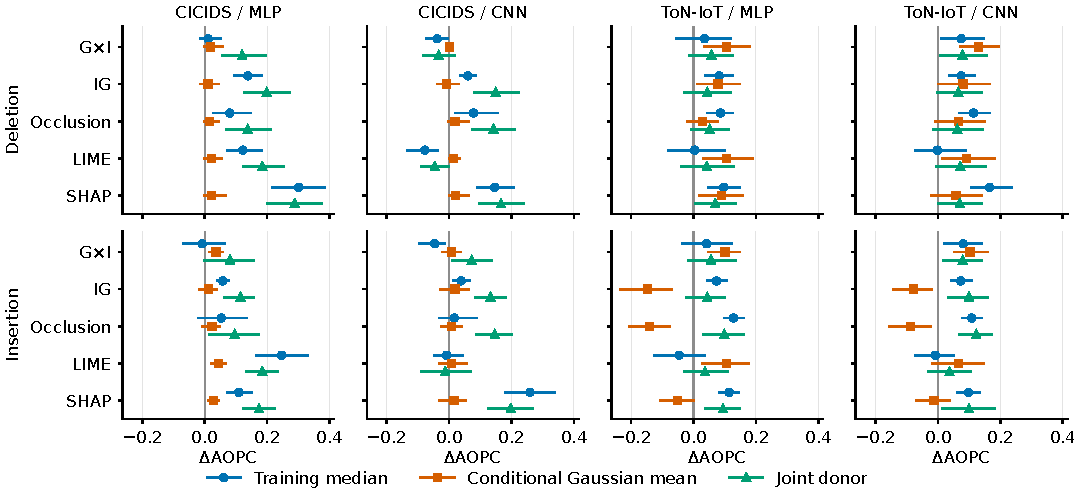
\includegraphics[width=\textwidth]{assets/binary_operators.pdf}
\caption{RQ2: attribution-minus-displacement-matched-random AOPC for deletion
(top) and insertion (bottom). Points are equal-seed means; bars are marginal
95\% source/seed intervals. Each task uses the same 80 distinct sources across
all methods, models and operators (16 per seed). Accounts and targets stay
fixed. Intervals condition on stored accounts, feature-index tie breaking and
intervention draws;
the three operators were selected for their different replacement mechanisms.}
\label{fig:operators}
\end{figure*}

\subsection{Aggregation and Scope of Uncertainty}

We average within each source/seed, then weight the five fitted seeds equally.
The 95\% intervals cross-resample source identities and seeds, preserving
source reuse; new conditional estimates and within-source operator contrasts
use 5,000 replicates. LIME intervals additionally retain the shared-run
jackknife treatment of its dependent pairwise comparisons. SHAP intervals
are conditional on two observed runs, not an estimated run population.
Existing cell intervals are retained only after independently reconstructing
the identical estimand and support. No interval is obtained by averaging
previous bounds. Functional intervals condition on frozen accounts and random
controls; they exclude fresh explainer/operator-draw variability. Comparisons
are exploratory, with marginal rather than multiplicity-adjusted intervals.
The version-matched repository package records source/seed identities,
configurations, hashes, exclusions and paired contrasts. Its reproduction
instructions rebuild Table~\ref{tab:repeatability} and both figures from the
included per-source records without model calls. A separate command
reconstructs the sensitivity summaries from their source-level measurements.
The package distinguishes recorded, reconstructed and unknown SHAP provenance.
Multiclass results do not enter the reported aggregates.
